\notechapter{N-20240518}{Projective Geometry: Homogeneous Coordinates, Infinity, and Duality}

\section{Why add points at infinity}

In the Euclidean plane, two nonparallel lines meet, but parallel lines do not. Projective geometry removes this exception. Parallel lines meet at a point at infinity.

This is not merely a trick for drawing perspective. It makes geometry cleaner: incidence statements no longer need special cases.

The guiding principle is:
\[
  \text{projective geometry prefers incidence over distance.}
\]
Lengths and angles are not the basic objects. Points, lines, and their incidence relations are.

\section{The projective line}

The projective line over a field \(k\) is
\[
  \mathbb P^1(k)=\{[x:y]:(x,y)\ne(0,0)\}/\sim,
\]
where
\[
  [x:y]=[\lambda x:\lambda y]\qquad(\lambda\ne0).
\]
The pair \([x:y]\) is a homogeneous coordinate. It does not describe a point of \(k^2\); it describes a line through the origin in \(k^2\).

The affine chart \(y\ne0\) identifies most points with numbers:
\[
  [x:y]=[x/y:1].
\]
The remaining point is \([1:0]\), the point at infinity.

\section{The projective plane}

The projective plane is
\[
  \mathbb P^2(k)=\{[x:y:z]:(x,y,z)\ne(0,0,0)\}/\sim.
\]
The affine chart \(z\ne0\) gives ordinary coordinates
\[
  [x:y:z]=[x/z:y/z:1].
\]
The line at infinity is the set \(z=0\). Thus the affine plane is not discarded. It becomes one chart inside a larger geometry.

\section{Lines and incidence}

A projective line in \(\mathbb P^2\) is given by a homogeneous linear equation
\[
  ax+by+cz=0.
\]
The coefficients \([a:b:c]\) themselves are homogeneous. Multiplying them by a nonzero scalar gives the same line.

Two distinct projective lines always meet. Algebraically, solving two independent homogeneous linear equations in three variables gives a one-dimensional solution space, hence a projective point.

For example, the affine parallel lines \(y=0\) and \(y=1\) become
\[
  y=0,\qquad y-z=0.
\]
At infinity \(z=0\), both contain the point \([1:0:0]\).

\section{Duality}

A point has coordinates \([x:y:z]\). A line has coordinates \([a:b:c]\). Incidence is the equation
\[
  ax+by+cz=0.
\]
This symmetry suggests projective duality: theorems about points and lines often have dual versions obtained by exchanging the words point and line.

\[
\begin{array}{c|c}
\text{statement} & \text{dual statement}\\
\hline
\text{two points determine a line} & \text{two lines determine a point}\\
\text{points lie on a line} & \text{lines pass through a point}
\end{array}
\]

\section{Projective transformations}

An invertible linear map \(A:k^3\to k^3\) sends lines through the origin to lines through the origin. Therefore it induces a transformation of \(\mathbb P^2\):
\[
  [v]\longmapsto [Av].
\]
These are projective transformations.

They preserve incidence, but not distances or angles. This is why circles may become ellipses in perspective drawings, while straight lines remain straight.

\section{Conics projectively}

A conic in the projective plane is given by a homogeneous quadratic equation
\[
  X^TAX=0,
\]
where \(X=(x,y,z)^T\) and \(A\) is a symmetric matrix. In affine coordinates \(z=1\), this becomes the usual quadratic equation in \(x\) and \(y\).

The projective viewpoint explains why ellipses, parabolas, and hyperbolas belong to one family. They are different affine shadows of projective conics.

%% expanded-on-review

\section{A picture of affine charts}

The projective plane is covered by three standard affine charts:
\[
  U_x=\{x\ne0\},\qquad U_y=\{y\ne0\},\qquad U_z=\{z\ne0\}.
\]
The usual affine plane is only the chart \(U_z\). Points on the line at infinity are not mysterious; they are simply points that do not appear in this chosen chart.

\begin{center}
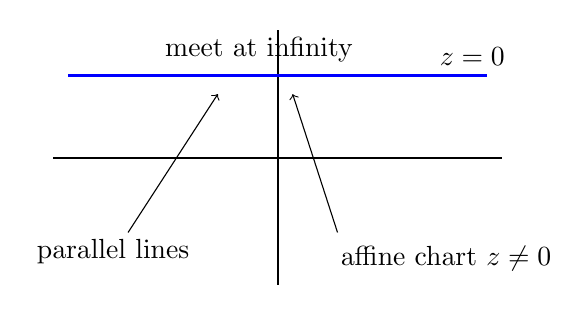
\begin{tikzpicture}[scale=0.95]
  \draw[thick] (-3,0) -- (3,0);
  \draw[thick] (0,-1.7) -- (0,1.7);
  \draw[very thick,blue] (-2.8,1.1) -- (2.8,1.1);
  \node at (2.6,1.35) {$z=0$};
  \node at (2.25,-1.35) {affine chart $z\ne0$};
  \draw[->] (-2,-1) -- (-.8,.85);
  \draw[->] (.8,-1) -- (.2,.85);
  \node at (-2.2,-1.25) {parallel lines};
  \node at (-.25,1.45) {meet at infinity};
\end{tikzpicture}
\end{center}

The diagram is deliberately schematic. The line at infinity is not physically above the plane; it is a projective completion of the affine picture.

\section{The cross-ratio as a first invariant}

Projective transformations do not preserve length, angle, or ordinary ratios of distances. But they do preserve one important quantity on a projective line: the cross-ratio.

For four points \(a,b,c,d\) on an affine coordinate line, define
\[
  [a,b;c,d]=\frac{(c-a)(d-b)}{(c-b)(d-a)}.
\]
This expression is unchanged under projective transformations of \(\mathbb P^1\).

The point of mentioning it here is not to develop a full theory of projective invariants. It is to show the change in taste: once distances are no longer meaningful, geometry searches for different invariants.

\section{Perspective as projective geometry}

A camera image is not an isometry of the world. It does not preserve lengths. But it sends straight lines to straight lines and preserves incidence. This is why projective geometry is the natural language of perspective.

Parallel railway tracks appear to meet at a vanishing point. In Euclidean geometry this is an illusion. In projective geometry it is exactly what the completed plane says should happen.


\section{What to remember}

Projective geometry is not harder because it adds infinity. It is easier because it removes exceptions.

\[
\begin{array}{c|c}
\text{affine habit} & \text{projective correction}\\
\hline
\text{parallel lines do not meet} & \text{they meet at infinity}\\
\text{coordinates are numbers} & \text{coordinates are ratios}\\
\text{line equations are separate from points} & \text{points and lines are dual}\\
\text{conics split into types} & \text{conics are one projective family}
\end{array}
\]
